% Source: Fukuda (2026), Supplementary Ch. 16 "Introduction to Continuous-Time
% Dynamic Optimization" (pp. 563-575): Sec. 16.1 (the continuous-time cake-eating
% problem solved by a direct variation, and the transversality condition that
% pins down the constant); Sec. 16.2 (the optimal-control problem, the
% present-value Hamiltonian and the three first-order conditions with their
% derivation by perturbation and integration by parts, the current-value
% Hamiltonian and the change mu = e^{rt} lambda, and the cake-eating example
% solved with both Hamiltonians); Sec. 16.3 (the calculus-of-variations problem,
% the Euler-Lagrange equation, its derivation from optimal control and its direct
% derivation); Sec. 16.4 and Example 16.1 (the heuristic continuous-time limit of
% the Bellman equation and the resulting HJB equation, solved for the cake
% problem by guess and verify). Proposition 7.30 (p. 288), the fundamental lemma
% of the calculus of variations, is the tool used throughout.
% No external reference is cited in this chapter, and no Gerzensee slide covers
% its material: every statement is drawn from the supplementary lecture notes
% listed above. The connection to the slides runs through the discrete-time
% Ramsey model of Dynamic Programming slides 36-41, treated in lec_15.tex.

\chapter{Continuous-Time Dynamic Optimisation}
\label{ch:continuoustime}

\section{From Sequences to Paths}\label{sec:ct-motivation}

The chapter preceding treated the choice of a sequence; this one treats the choice
of a function of time. The change is not merely notational. A sequence is a point
in a space of countably many coordinates and can be perturbed one coordinate at a
time; a path must be perturbed by another path, and the first-order condition is
therefore an equation that must hold for \emph{every} admissible perturbation.
Converting such a family of scalar conditions into a pointwise differential
equation is the office of the following lemma, and every result in this chapter
rests on it.

\begin{lemma}[Fundamental lemma of the calculus of variations]\label{lem:fundamental-cov}
	Let $t_0<t_1$ and let $g\in\Cspace{[t_0,t_1]}{\R}$ satisfy
	\begin{equation}\label{eq:fundamental-cov}
		\int_{t_0}^{t_1}g(t)h(t)\,\diff t=0
		\qquad\text{for every }h\in\Cspace{[t_0,t_1]}{\R}
		\text{ with }h(t_0)=h(t_1)=0 .
	\end{equation}
	Then $g\equiv0$ on $[t_0,t_1]$.
\end{lemma}

\begin{proof}
	Suppose $g(s)\neq0$ for some $s\in(t_0,t_1)$; without loss of generality
	$g(s)>0$, otherwise replace $g$ by $-g$. By continuity there are
	$\alpha,\beta$ with $t_0<\alpha<s<\beta<t_1$ and
	$g(t)>\tfrac12g(s)$ for every $t\in[\alpha,\beta]$. Define
	\[
		h(t)\eqdef\begin{cases}(t-\alpha)(\beta-t), & t\in[\alpha,\beta], \\
              0,                            & \text{otherwise.}\end{cases}
	\]
	This $h$ is continuous on $[t_0,t_1]$ --- it vanishes at $\alpha$ and $\beta$,
	where the two branches meet --- non-negative, and satisfies
	$h(t_0)=h(t_1)=0$. Then
	\[
		\int_{t_0}^{t_1}g(t)h(t)\,\diff t
		=\int_{\alpha}^{\beta}g(t)h(t)\,\diff t
		>\frac{g(s)}{2}\int_{\alpha}^{\beta}(t-\alpha)(\beta-t)\,\diff t
		=\frac{g(s)}{2}\cdot\frac{(\beta-\alpha)^{3}}{6}>0,
	\]
	using \autoref{prop:integral-properties} for the strict monotonicity of the
	integral of a continuous function that is strictly positive on
	$[\alpha,\beta]$. This contradicts \eqref{eq:fundamental-cov}. Hence $g$
	vanishes on the open interval, and by continuity at the endpoints as well.
\end{proof}

This is Proposition~7.30 of \textcite[p.~288]{fukuda2026notes}. Read in the
language of \autoref{ch:projection}, it says that the only continuous function
orthogonal, in the $L^{2}$ inner product $\ip{g}{h}=\int g h$, to every continuous
function vanishing at the endpoints is the zero function: the set of such $h$ is
dense in $L^{2}[t_0,t_1]$, so its orthogonal complement is trivial by
\autoref{prop:orthogonal-complement}. The elementary proof above avoids the
density argument and is the one used here because it also delivers the conclusion
for the piecewise-defined perturbations that appear in constrained problems.

\section{The Calculus of Variations}\label{sec:ct-variations}

\begin{definition}[Variational problem]\label{def:variational-problem}
	Given $f\colon[t_0,t_1]\times\R\times\R\to\R$ continuously differentiable and
	endpoints $x_0,x_1\in\R$, the \dfnas{calculus-of-variations
		problem}{calculus of variations} is
	\begin{equation}\label{eq:cov-problem}
		\max_{x(\cdot)}\ \int_{t_0}^{t_1}f\bigl(t,x(t),\dot x(t)\bigr)\,\diff t
		\qquad\st\quad x(t_0)=x_0,\ x(t_1)=x_1,
	\end{equation}
	the maximum being over continuously differentiable paths $x\colon[t_0,t_1]\to\R$.
\end{definition}

\begin{theorem}[Euler--Lagrange equation]\label{thm:euler-lagrange}
	Let $x^{\ast}$ solve \eqref{eq:cov-problem} and suppose
	$t\mapsto f_{\dot x}\bigl(t,x^{\ast}(t),\dot x^{\ast}(t)\bigr)$ is continuously
	differentiable. Then
	\begin{equation}\label{eq:euler-lagrange}
		f_x\bigl(t,x^{\ast}(t),\dot x^{\ast}(t)\bigr)
		-\deriv{}{t}\Bigl[f_{\dot x}\bigl(t,x^{\ast}(t),\dot x^{\ast}(t)\bigr)\Bigr]=0
		\qquad\text{for every }t\in[t_0,t_1].
	\end{equation}
\end{theorem}

\begin{proof}
	Fix a continuously differentiable $h$ with $h(t_0)=h(t_1)=0$, so that
	$x^{\ast}+ah$ is admissible for every $a\in\R$, and set
	\[
		J(a)\eqdef\int_{t_0}^{t_1}
		f\bigl(t,x^{\ast}(t)+ah(t),\dot x^{\ast}(t)+a\dot h(t)\bigr)\,\diff t .
	\]
	Optimality of $x^{\ast}$ gives $J(0)\geq J(a)$ for all $a$, so $a=0$ is an
	interior maximiser of $J$ and \autoref{thm:fermat} gives $J'(0)=0$, provided
	$J$ is differentiable. It is, by
	\autoref{thm:differentiation-under-integral}: the integrand is continuously
	differentiable in $a$ and its $a$-derivative is continuous in $(t,a)$, hence
	bounded on the compact set $[t_0,t_1]\times[-1,1]$. Differentiating under the
	integral sign and using \autoref{thm:chain-rule},
	\[
		J'(a)=\int_{t_0}^{t_1}\Bigl\{f_x\bigl(t,x,\dot x\bigr)h(t)
		+f_{\dot x}\bigl(t,x,\dot x\bigr)\dot h(t)\Bigr\}\,\diff t,
		\qquad x=x^{\ast}+ah .
	\]
	Integrating the second term by parts (\autoref{thm:by-parts}),
	\[
		\int_{t_0}^{t_1}f_{\dot x}\dot h\,\diff t
		=\at{f_{\dot x}h}{t_0}{t_1}
		-\int_{t_0}^{t_1}\deriv{f_{\dot x}}{t}h\,\diff t
		=-\int_{t_0}^{t_1}\deriv{f_{\dot x}}{t}h\,\diff t,
	\]
	the boundary term vanishing because $h(t_0)=h(t_1)=0$. Hence
	\[
		0=J'(0)=\int_{t_0}^{t_1}
		\Bigl[f_x\bigl(t,x^{\ast},\dot x^{\ast}\bigr)
			-\deriv{}{t}f_{\dot x}\bigl(t,x^{\ast},\dot x^{\ast}\bigr)\Bigr]h(t)\,\diff t
	\]
	for every admissible $h$, and \autoref{lem:fundamental-cov} gives
	\eqref{eq:euler-lagrange}.
\end{proof}

The derivative $\deriv{}{t}f_{\dot x}$ in \eqref{eq:euler-lagrange} is a total
derivative along the path, not a partial derivative: expanded by the chain rule
it is
$f_{\dot xt}+f_{\dot xx}\dot x^{\ast}+f_{\dot x\dot x}\ddot x^{\ast}$, so the
Euler--Lagrange equation is a second-order ordinary differential equation in
$x^{\ast}$, and the two endpoint conditions of \eqref{eq:cov-problem} are exactly
what a second-order equation requires. That count is the structural reason a
variational problem with one free endpoint needs a substitute boundary condition,
and the substitute is the transversality condition of
\autoref{sec:ct-control}.

\begin{remark}[Necessary, not sufficient]\label{rem:el-necessary}
	\autoref{thm:euler-lagrange} is a first-order necessary condition and nothing
	more: it is \autoref{thm:fermat} applied along a one-parameter family, so it
	identifies stationary paths, among which are minima and saddles. Sufficiency
	requires concavity, exactly as in \autoref{thm:foc-concave}. If
	$(x,\dot x)\mapsto f(t,x,\dot x)$ is concave for each $t$, then a path
	satisfying \eqref{eq:euler-lagrange} is a global maximiser, because for any
	admissible $x$,
	\[
		\int_{t_0}^{t_1}\bigl[f(t,x,\dot x)-f(t,x^{\ast},\dot x^{\ast})\bigr]\,\diff t
		\leq\int_{t_0}^{t_1}\bigl[f_x\cdot(x-x^{\ast})
			+f_{\dot x}\cdot(\dot x-\dot x^{\ast})\bigr]\,\diff t=0,
	\]
	the inequality by \autoref{thm:concave-gradient} and the final equality by the
	same integration by parts as in the proof, using \eqref{eq:euler-lagrange} and
	$x(t_i)=x^{\ast}(t_i)$. The concavity hypothesis is satisfied in the economic
	problems below because $U$ is concave and the constraint is linear in the
	control.
\end{remark}

\section{Optimal Control}\label{sec:ct-control}

Optimal control generalises \autoref{def:variational-problem} by separating the
control from the rate of change of the state, which permits constraints on the
control and transitions that are not of the form $\dot x=u$.

\begin{definition}[Optimal control problem]\label{def:control-problem}
	Given $f$ and $g$ continuously differentiable,
	\begin{equation}\label{eq:control-problem}
		\max_{u(\cdot)}\ \int_{t_0}^{t_1}f\bigl(t,x(t),u(t)\bigr)\,\diff t
		\qquad\st\quad
		\dot x(t)=g\bigl(t,x(t),u(t)\bigr),\quad x(t_0)=x_0 .
	\end{equation}
	The function $x$ is the \dfn{state}, $u$ the \dfn{control}, and the
	\dfnas{present-value Hamiltonian}{Hamiltonian} is
	\begin{equation}\label{eq:hamiltonian}
		\mathcal{H}(t,x,u,\lambda)\eqdef f(t,x,u)+\lambda(t)\,g(t,x,u),
	\end{equation}
	with $\lambda$ the \dfnas{co-state variable}{co-state variable}.
	\nidx{hamiltonian}{$\mathcal{H}$, Hamiltonian}
\end{definition}

\begin{theorem}[Maximum principle, interior case]\label{thm:maximum-principle}
	Let $(u^{\ast},x^{\ast})$ solve \eqref{eq:control-problem} with $t_1<\infty$ and
	$x(t_1)$ free, and suppose $u^{\ast}$ is interior to the set of admissible
	controls. Then there is a continuously differentiable
	$\lambda\colon[t_0,t_1]\to\R$ such that, for every $t$,
	\begin{align}
		\pderiv{\mathcal{H}}{u}=0
		 & \iff f_u+\lambda g_u=0,\label{eq:mp-optimality}                     \\
		-\pderiv{\mathcal{H}}{x}=\dot\lambda
		 & \iff \dot\lambda(t)=-\bigl(f_x+\lambda g_x\bigr),\label{eq:mp-costate} \\
		\pderiv{\mathcal{H}}{\lambda}=\dot x
		 & \iff \dot x=g,\label{eq:mp-state}
	\end{align}
	together with the initial condition $x(t_0)=x_0$ and the
	\dfnas{transversality condition}{transversality condition} $\lambda(t_1)=0$.
\end{theorem}

\begin{proof}
	Perturb the control, $u=u^{\ast}+ah$ for a fixed continuously differentiable
	$h$, and let $y(t,a)$ be the state path it induces through
	\eqref{eq:mp-state}, so $y(t,0)=x^{\ast}(t)$ and $y(t_0,a)=x_0$ for every $a$.
	Let $\lambda$ be any continuously differentiable function, to be chosen. Since
	the constraint holds identically along every admissible path, the objective is
	unchanged by adding $\lambda(g-\dot x)\equiv0$ to the integrand, and
	integration by parts (\autoref{thm:by-parts}) gives
	\begin{align*}
		J(a) & \eqdef\int_{t_0}^{t_1}
		\Bigl\{f\bigl(t,y,u^{\ast}+ah\bigr)
		+\lambda g\bigl(t,y,u^{\ast}+ah\bigr)-\lambda\dot y\Bigr\}\,\diff t                        \\
		     & =\int_{t_0}^{t_1}\Bigl\{f+\lambda g+\dot\lambda\,y\Bigr\}\,\diff t
		-\lambda(t_1)y(t_1,a)+\lambda(t_0)\underbrace{y(t_0,a)}_{=x_0} .
	\end{align*}
	Differentiating at $a=0$, legitimate by
	\autoref{thm:differentiation-under-integral}, and writing
	$y_a\eqdef\partial y/\partial a$ evaluated at $a=0$,
	\begin{equation}\label{eq:mp-variation}
		J'(0)=\int_{t_0}^{t_1}
		\Bigl\{\bigl(f_u+\lambda g_u\bigr)h
		+\bigl(f_x+\lambda g_x+\dot\lambda\bigr)y_a\Bigr\}\,\diff t
		-\lambda(t_1)\,y_a(t_1),
	\end{equation}
	the term in $\lambda(t_0)$ contributing nothing because $y(t_0,a)=x_0$ for all
	$a$.

	The function $\lambda$ is still free. Choose it to solve the linear differential
	equation \eqref{eq:mp-costate} with terminal condition $\lambda(t_1)=0$; a
	solution exists and is unique on $[t_0,t_1]$ because the equation is linear in
	$\lambda$ with continuous coefficients, and the integrating-factor
	representation
	$\lambda(t)=\int_{t}^{t_1}f_x(s)\exp\bigl(\int_{t}^{s}g_x(\tau)\,\diff\tau\bigr)\,\diff s$
	exhibits it. This choice annihilates the second and third terms of
	\eqref{eq:mp-variation}, and $J'(0)=0$ by optimality, leaving
	\[
		\int_{t_0}^{t_1}\bigl(f_u+\lambda g_u\bigr)h(t)\,\diff t=0
		\qquad\text{for every admissible }h .
	\]
	\autoref{lem:fundamental-cov} then gives \eqref{eq:mp-optimality} pointwise.
	Equation \eqref{eq:mp-state} is the constraint, restated as a partial derivative
	of $\mathcal{H}$.
\end{proof}

\begin{remark}[What the three conditions say]\label{rem:mp-reading}
	The co-state $\lambda(t)$ is the shadow price of the state at time $t$, the
	continuous-time counterpart of the multiplier of \autoref{thm:kuhn-tucker} and
	of the derivative $V'(x)$ of \autoref{thm:euler-envelope}. The optimality
	condition \eqref{eq:mp-optimality} equates the marginal current return of the
	control to its marginal cost in terms of the state it consumes, valued at
	$\lambda$. The co-state equation \eqref{eq:mp-costate} is an asset-pricing
	condition: rearranged as $-\dot\lambda=f_x+\lambda g_x$, it says the capital loss
	on a unit of the state equals its current dividend plus its contribution to
	future accumulation. The transversality condition $\lambda(t_1)=0$ says a unit
	of the state has no value at the terminal date when the terminal state is free:
	anything left over is wasted, so nothing should be left over.

	When $t_1=\infty$ the terminal condition must be replaced. The standard form is
	$\lim_{t\to\infty}\lambda(t)x(t)=0$ in present-value terms, or
	$\lim_{t\to\infty}e^{-\rho t}\mu(t)x(t)=0$ in current-value terms, and
	\autoref{sec:ct-cake} shows what goes wrong without it: the first-order
	conditions leave a free constant that only the transversality condition pins
	down.
\end{remark}

\begin{proposition}[Current-value Hamiltonian]\label{prop:current-value}
	Consider the discounted problem
	\begin{equation}\label{eq:discounted-control}
		\max_{u(\cdot)}\ \int_{t_0}^{t_1}e^{-\rho t}f\bigl(t,x(t),u(t)\bigr)\,\diff t
		\qquad\st\quad\dot x=g(t,x,u),\ x(t_0)=x_0,
	\end{equation}
	and define the \dfnas{current-value Hamiltonian}{current-value Hamiltonian}
	$H\eqdef e^{\rho t}\mathcal{H}=f(t,x,u)+\mu(t)g(t,x,u)$ with
	$\mu(t)\eqdef e^{\rho t}\lambda(t)$. Then \eqref{eq:mp-optimality}--%
	\eqref{eq:mp-state} become
	\begin{equation}\label{eq:current-value-conditions}
		\pderiv{H}{u}=0,
		\qquad
		\dot\mu(t)=\rho\mu(t)-\pderiv{H}{x},
		\qquad
		\pderiv{H}{\mu}=\dot x .
	\end{equation}
\end{proposition}

\begin{proof}
	The optimality condition is unaffected by multiplying $\mathcal{H}$ by the
	positive factor $e^{\rho t}$, which does not depend on $u$. For the co-state
	equation, \eqref{eq:mp-costate} reads
	$-\dot\lambda=\partial\mathcal{H}/\partial x$, and multiplying by $e^{\rho t}$
	gives $-e^{\rho t}\dot\lambda=\partial H/\partial x$. Since
	$\mu=e^{\rho t}\lambda$, the product rule
	(\autoref{prop:deriv-product}) gives
	\[
		\dot\mu=\rho e^{\rho t}\lambda+e^{\rho t}\dot\lambda
		=\rho\mu-\pderiv{H}{x} .
	\]
	The state equation is unchanged since $\partial H/\partial\mu=g$.
\end{proof}

The current-value formulation removes the explicit $e^{-\rho t}$ from every
equation and leaves an autonomous system whenever $f$ and $g$ do not depend on
$t$ directly. That is the practical reason it is preferred in economics: the
resulting pair of differential equations in $(x,\mu)$ has a phase diagram, and
the steady state and saddle path of \autoref{sec:ct-ramsey} are features of that
diagram.

\begin{proposition}[Calculus of variations as a special case]\label{prop:cov-from-control}
	The problem \eqref{eq:cov-problem} is \eqref{eq:control-problem} with
	$u\eqdef\dot x$ and $g(t,x,u)=u$, and the maximum principle then reproduces the
	Euler--Lagrange equation \eqref{eq:euler-lagrange}.
\end{proposition}

\begin{proof}
	With $g=u$ the Hamiltonian is $\mathcal{H}=f(t,x,u)+\lambda u$, so
	\eqref{eq:mp-optimality} reads $f_u+\lambda=0$ and \eqref{eq:mp-costate} reads
	$\dot\lambda=-f_x$. Differentiating the first along the path and using
	$u=\dot x$ from \eqref{eq:mp-state},
	\[
		\dot\lambda=-\deriv{}{t}f_u\bigl(t,x,u\bigr)
		=-\deriv{}{t}f_{\dot x}\bigl(t,x,\dot x\bigr),
	\]
	and eliminating $\dot\lambda$ between this and $\dot\lambda=-f_x$ gives
	$f_x=\deriv{}{t}f_{\dot x}$.
\end{proof}

\section{The Hamilton--Jacobi--Bellman Equation}\label{sec:ct-hjb}

The third route to the same conditions is dynamic programming, obtained as the
continuous-time limit of \autoref{ch:dynamic}.

\paragraph{Heuristic derivation.} Let the period length be $\delta>0$ and the
per-period discount factor $1/(1+\delta\rho)$. The discrete Bellman equation for
the value $W(t,x)$ of the problem started at date $t$ in state $x$ is
\[
	W(t,x)=\max_{u}\ \Bigl\{\Bigl(\tfrac{1}{1+\delta\rho}\Bigr)^{\delta t}
	r(x,u)\,\delta+W\bigl(t+\delta,\,x+g(x,u)\delta\bigr)\Bigr\},
\]
the state moving by $g(x,u)\delta$ over an interval of length $\delta$. Assuming
$W$ differentiable and expanding to first order by \autoref{thm:taylor-n},
\[
	W\bigl(t+\delta,x+g\delta\bigr)
	=W(t,x)+W_t(t,x)\delta+W_x(t,x)g(x,u)\delta+o(\delta).
\]
Substituting, cancelling $W(t,x)$, dividing by $\delta$ and letting
$\delta\downarrow0$ --- using
$\lim_{\delta\to0}(1+\delta\rho)^{-\delta t/\delta}
	=\lim_{\delta\to0}(1+\delta\rho)^{-\rho t/(\delta\rho)}=e^{-\rho t}$ --- gives
\[
	0=W_t(t,x)+\max_u\bigl\{e^{-\rho t}r(x,u)+W_x(t,x)g(x,u)\bigr\}.
\]
Stationarity makes $W(t,x)=e^{-\rho t}V(x)$ where
$V(x)\eqdef\max\int_0^{\infty}e^{-\rho t}r(x_t,u_t)\,\diff t$ from $x_0=x$; then
$W_t=-\rho e^{-\rho t}V(x)$ and $W_x=e^{-\rho t}V'(x)$, and dividing through by
$e^{-\rho t}$ leaves the following.

\begin{definition}[HJB equation]\label{def:hjb}
	The \dfnas{Hamilton--Jacobi--Bellman equation}{Hamilton--Jacobi--Bellman
		equation} of the stationary infinite-horizon problem
	$V(x)=\max\int_0^{\infty}e^{-\rho t}r(x_t,u_t)\,\diff t$ subject to
	$\dot x=g(x,u)$, $x_0=x$, is
	\begin{equation}\label{eq:hjb}
		\rho V(x)=\max_{u}\ \bigl\{r(x,u)+V'(x)\,g(x,u)\bigr\}.
	\end{equation}
\end{definition}

Equation \eqref{eq:hjb} is the asset-pricing form of the Bellman equation and was
met in \eqref{eq:hjb-scalar}: the required return $\rho V$ on the ``asset'' $x$
equals the current dividend $r$ plus the expected capital gain
$V'(x)\dot x$. Comparing \eqref{eq:hjb} with \eqref{eq:hamiltonian} identifies
the maximand as the current-value Hamiltonian with $\mu=V'(x)$: the co-state is
the derivative of the value function, exactly as $\lambda$ was the shadow price in
\autoref{rem:mp-reading} and as $V'$ was in \eqref{eq:ramsey-envelope}. The three
methods of this chapter --- variations, the maximum principle, dynamic programming
--- are therefore three presentations of one set of conditions, and which is most
convenient depends on the problem rather than on the mathematics.

\begin{remark}[The status of the derivation]\label{rem:hjb-heuristic}
	The passage to the limit above assumes what it should prove: that $W$ is
	differentiable, that the limit and the maximum interchange, and that the
	discrete problems converge to the continuous one. None of these is automatic.
	The value function of a control problem is in general only continuous, and
	\eqref{eq:hjb} then holds in the weaker \emph{viscosity} sense rather than
	pointwise. Where a classical solution of \eqref{eq:hjb} does exist and the
	associated policy is admissible, a verification argument establishes optimality
	directly, without any limit: this is the content of
	\autoref{prop:ct-cake-verification} below, and it is why guess-and-verify is the
	honest way to use \eqref{eq:hjb}.
\end{remark}

\section{The Continuous-Time Cake-Eating Problem}\label{sec:ct-cake}

\paragraph{Problem.} Maximise $\int_0^{\infty}e^{-rt}\log c(t)\,\diff t$ subject to
$\dot k(t)=-c(t)$, $k(0)=k_0>0$, $c(t)>0$, together with the transversality
condition $\lim_{t\to\infty}k(t)=0$.

\begin{proposition}[Solution by three routes]\label{prop:ct-cake}
	The problem has the unique solution
	\begin{equation}\label{eq:ct-cake-solution}
		k^{\ast}(t)=k_0e^{-rt},
		\qquad
		c^{\ast}(t)=rk_0e^{-rt},
		\qquad
		V(k)=\frac{\log r-1+\log k}{r},
	\end{equation}
	and the optimal feedback rule is $c=rk$.
\end{proposition}

\begin{proof}
	\emph{Variational route.} Substituting $c=-\dot k$ turns the problem into
	\eqref{eq:cov-problem} with $f(t,k,\dot k)=e^{-rt}\log(-\dot k)$. Here $f_k=0$
	and $f_{\dot k}=-e^{-rt}/(-\dot k)\cdot(-1)=e^{-rt}/\dot k$, so
	\eqref{eq:euler-lagrange} reduces to
	\[
		\deriv{}{t}\left(\frac{e^{-rt}}{\dot k^{\ast}(t)}\right)=0,
	\]
	that is $e^{-rt}/\dot k^{\ast}(t)$ is constant in $t$, so
	$\dot k^{\ast}(t)=ae^{-rt}$ for some $a\in\R$. Integrating from $0$ to $t$ by
	\autoref{thm:ftc},
	\[
		k^{\ast}(t)=k_0+\int_0^{t}ae^{-r\tau}\,\diff\tau
		=k_0+\frac{a}{r}\bigl(1-e^{-rt}\bigr).
	\]
	Letting $t\to\infty$ and imposing $\lim_tk^{\ast}(t)=0$ gives
	$k_0+a/r=0$, that is $a=-rk_0$, whence
	$k^{\ast}(t)=k_0e^{-rt}$ and $c^{\ast}(t)=-\dot k^{\ast}(t)=rk_0e^{-rt}$.

	\emph{Hamiltonian route.} The current-value Hamiltonian is
	$H=\log c-\mu c$. Condition \eqref{eq:current-value-conditions} gives
	$1/c=\mu$; and $\partial H/\partial k=0$, so $\dot\mu=r\mu$. This separable
	equation integrates to $\mu(t)=\mu(0)e^{rt}$, hence
	$c(t)=1/\mu(t)=ae^{-rt}$ with $a=1/\mu(0)$. The state equation and the
	transversality condition then reproduce the previous paragraph with the
	sign of $a$ reversed, giving $a=rk_0$ and the same paths. With the
	present-value Hamiltonian $\mathcal{H}=e^{-rt}\log c-\lambda c$ the co-state
	equation is $-\dot\lambda=\partial\mathcal{H}/\partial k=0$, so $\lambda$ is
	constant and $e^{-rt}/c(t)=\lambda$ delivers $c(t)=ae^{-rt}$ directly.

	\emph{Dynamic programming route.} See
	\autoref{prop:ct-cake-verification}.
\end{proof}

\begin{proposition}[Verification via HJB]\label{prop:ct-cake-verification}
	The function $V(k)=(\log r-1+\log k)/r$ solves \eqref{eq:hjb} for the
	cake problem, the maximiser is $c=rk$, and the resulting path is optimal.
\end{proposition}

\begin{proof}
	Here $r(k,c)=\log c$ and $g(k,c)=-c$, so \eqref{eq:hjb} reads
	$rV(k)=\max_{c>0}\{\log c-V'(k)c\}$. Guess $V(k)=A+B\log k$, so
	$V'(k)=B/k>0$ for $B>0$; the objective is then strictly concave in $c$ with
	$\lim_{c\downarrow0}$ derivative $+\infty$, so by \autoref{thm:foc-concave} the
	unique maximiser solves $1/c=B/k$, that is $c=k/B$. Substituting,
	\[
		r(A+B\log k)=\log\frac{k}{B}-\frac{B}{k}\cdot\frac{k}{B}
		=\log k-\log B-1 .
	\]
	Matching the coefficient of $\log k$ gives $rB=1$, so $B=1/r$; matching
	constants gives $rA=-\log B-1=\log r-1$, so $A=(\log r-1)/r$. The feedback rule
	is $c=k/B=rk$, so the state obeys $\dot k=-rk$, giving
	$k^{\ast}(t)=k_0e^{-rt}$ and $c^{\ast}(t)=rk_0e^{-rt}$, which satisfy the
	transversality condition.

	For optimality, let $(c,k)$ be any admissible path. Since $V$ is concave,
	\autoref{thm:concave-gradient} and the HJB equation give, for every $t$,
	\[
		\deriv{}{t}\Bigl[e^{-rt}V\bigl(k(t)\bigr)\Bigr]
		=e^{-rt}\Bigl[V'(k)\dot k-rV(k)\Bigr]
		=e^{-rt}\Bigl[-V'(k)c-rV(k)\Bigr]
		\leq-e^{-rt}\log c(t),
	\]
	the inequality because $rV(k)\geq\log c-V'(k)c$ for every feasible $c$, by the
	maximum in \eqref{eq:hjb}. Integrating from $0$ to $T$,
	\[
		\int_0^{T}e^{-rt}\log c(t)\,\diff t\leq V(k_0)-e^{-rT}V\bigl(k(T)\bigr),
	\]
	and letting $T\to\infty$ along any path satisfying the transversality condition
	kills the last term, giving
	$\int_0^{\infty}e^{-rt}\log c\,\diff t\leq V(k_0)$, with equality along the
	candidate path because the inequality above is then an equality at every $t$.
\end{proof}

\begin{figure}[htbp]
	\centering
	% Figures/cake-paths.tex
% Optimal paths of the continuous-time cake-eating problem, Proposition
% \ref{prop:ct-cake} of Chapter \ref{ch:continuoustime}:
% k^*(t)=k_0e^{-rt} and c^*(t)=rk_0e^{-rt}, drawn for r=0.4 and k_0=1.
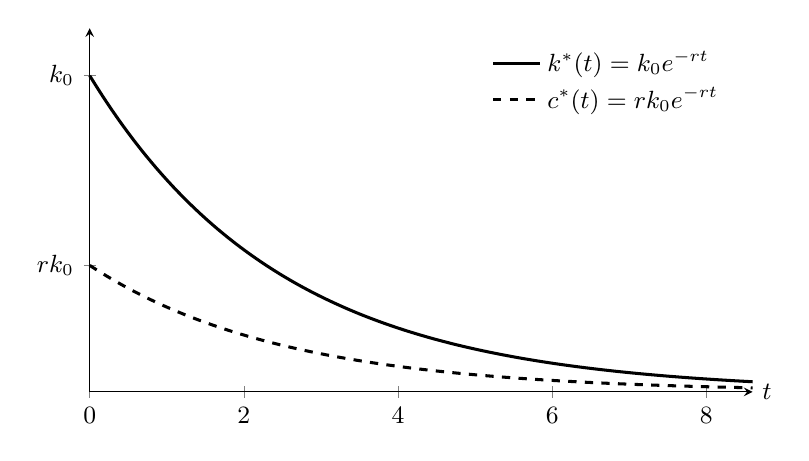
\begin{tikzpicture}
	\begin{axis}[
			width=10cm, height=6.2cm,
			axis lines=left,
			xlabel={$t$},
			every axis x label/.style={at={(current axis.right of origin)},anchor=west},
			xmin=0, xmax=8.6, ymin=0, ymax=1.15,
			xtick={0,2,4,6,8},
			ytick={0.4,1}, yticklabels={$rk_0$,$k_0$},
			tick label style={font=\small},
			label style={font=\small},
			legend cell align=left,
			legend style={draw=none, fill=none, font=\small,
					at={(0.97,0.97)}, anchor=north east},
			clip=false,
		]
		\addplot[line width=1.1pt, domain=0:8.6, samples=120] {exp(-0.4*x)};
		\addlegendentry{$k^{\ast}(t)=k_0e^{-rt}$}

		\addplot[line width=1.1pt, dashed, domain=0:8.6, samples=120]
		{0.4*exp(-0.4*x)};
		\addlegendentry{$c^{\ast}(t)=rk_0e^{-rt}$}
	\end{axis}
\end{tikzpicture}

	\caption[Optimal paths in the continuous-time cake problem]{The optimal
		paths \eqref{eq:ct-cake-solution}. Both decay at the common rate $r$, so
		the ratio $c^{\ast}(t)/k^{\ast}(t)$ is constant and equal to $r$: the
		feedback rule $c=rk$ is what makes the two curves scaled copies of each
		other. The cake is exhausted only in the limit, which is the content of
		the transversality condition $\lim_{t\to\infty}k(t)=0$.}
	\label{fig:cake-paths}
\end{figure}

\begin{remark}[The discrete-time limit]\label{rem:ct-discrete-limit}
	Compare \eqref{eq:ct-cake-solution}, drawn in \autoref{fig:cake-paths}, with
	\eqref{eq:cake-solution}. In discrete
	time with period length $\Delta$ and discount factor
	$\beta=e^{-r\Delta}$, the policy is $c=(1-\beta)w$ per period, so the
	consumption \emph{rate} is
	\[
		\frac{(1-e^{-r\Delta})w}{\Delta}\xrightarrow[\Delta\downarrow0]{}rw,
	\]
	by \autoref{thm:taylor-1d} applied to $\Delta\mapsto e^{-r\Delta}$, which is
	exactly the feedback rule $c=rk$. Correspondingly the cake decays at rate
	$\beta^{t/\Delta}=e^{-rt}$, matching $k^{\ast}(t)=k_0e^{-rt}$. The rate of time
	preference $r$ in continuous time and the discount factor $\beta$ in discrete
	time are related by $\beta=1/(1+r\Delta)+o(\Delta)$, which is the substitution
	made in the derivation of \eqref{eq:hjb}. The agreement is not automatic --- it
	requires the transversality conditions to correspond, which they do here
	because both take the form ``the state is asymptotically exhausted''.
\end{remark}

\section{The Ramsey Model in Continuous Time}\label{sec:ct-ramsey}

\paragraph{Problem.} A planner maximises
$\int_0^{\infty}e^{-\rho t}u(c(t))\,\diff t$ subject to
\begin{equation}\label{eq:ct-ramsey-constraint}
	\dot k(t)=f\bigl(k(t)\bigr)-\delta k(t)-c(t),
	\qquad k(0)=k_0>0,\ c(t)\geq0,\ k(t)\geq0,
\end{equation}
with $f$ strictly increasing, strictly concave and satisfying the Inada
conditions, $u$ strictly increasing, strictly concave and twice differentiable,
$\rho>0$ and $\delta\in[0,1]$.

\begin{theorem}[Keynes--Ramsey rule and the modified golden rule]\label{thm:keynes-ramsey}
	Along an interior optimal path of \eqref{eq:ct-ramsey-constraint},
	\begin{equation}\label{eq:keynes-ramsey}
		\frac{\dot c(t)}{c(t)}
		=\frac{f'\bigl(k(t)\bigr)-\delta-\rho}{\gamma\bigl(c(t)\bigr)},
		\qquad
		\gamma(c)\eqdef-\frac{c\,u''(c)}{u'(c)},
	\end{equation}
	and the unique interior steady state $(k^{\ast},c^{\ast})$ satisfies
	\begin{equation}\label{eq:modified-golden-rule}
		f'(k^{\ast})=\rho+\delta,
		\qquad
		c^{\ast}=f(k^{\ast})-\delta k^{\ast}.
	\end{equation}
\end{theorem}

\begin{proof}
	The current-value Hamiltonian is
	$H=u(c)+\mu\bigl(f(k)-\delta k-c\bigr)$. By
	\autoref{prop:current-value},
	\begin{equation}\label{eq:ct-ramsey-foc}
		\pderiv{H}{c}=u'(c)-\mu=0,
		\qquad
		\dot\mu=\rho\mu-\pderiv{H}{k}=\rho\mu-\mu\bigl(f'(k)-\delta\bigr)
		=\mu\bigl(\rho+\delta-f'(k)\bigr).
	\end{equation}
	Differentiating $u'(c)=\mu$ in $t$ by \autoref{prop:chain-rule-1d} gives
	$u''(c)\dot c=\dot\mu=u'(c)\bigl(\rho+\delta-f'(k)\bigr)$, so
	\[
		\frac{c\,u''(c)}{u'(c)}\cdot\frac{\dot c}{c}=\rho+\delta-f'(k),
		\qquad\text{that is}\qquad
		-\gamma(c)\frac{\dot c}{c}=\rho+\delta-f'(k),
	\]
	which is \eqref{eq:keynes-ramsey}. At a steady state $\dot c=0$, and since
	$\gamma(c)>0$ by strict concavity of $u$, the numerator must vanish:
	$f'(k^{\ast})=\rho+\delta$. Strict concavity of $f$ makes $f'$ strictly
	decreasing, and the Inada conditions make it range over $(0,\infty)$, so
	$k^{\ast}$ exists and is unique. Setting $\dot k=0$ in
	\eqref{eq:ct-ramsey-constraint} gives $c^{\ast}=f(k^{\ast})-\delta k^{\ast}$.
\end{proof}

\begin{remark}[Reading the Keynes--Ramsey rule]\label{rem:keynes-ramsey}
	Equation \eqref{eq:keynes-ramsey} decomposes consumption growth into a rate
	of return and a willingness to substitute. Consumption rises when the net
	marginal product of capital $f'(k)-\delta$ exceeds the rate of time preference
	$\rho$, and the responsiveness is the elasticity of intertemporal substitution
	$1/\gamma$. For CRRA utility $\gamma$ is constant and \eqref{eq:keynes-ramsey}
	is the continuous-time counterpart of \eqref{eq:ramsey-euler}; at
	$\rho=\beta^{-1}-1$ the two steady-state conditions
	$f'(k^{\ast})=\rho+\delta$ and $\beta\bigl(f'(k^{\ast})+1-\delta\bigr)=1$
	coincide, as they must.

	The modified golden rule places $k^{\ast}$ strictly below the golden-rule stock
	$k^{g}$ defined by $f'(k^{g})=\delta$, which maximises steady-state consumption
	$f(k)-\delta k$. The gap is impatience: a planner with $\rho=0$ would accumulate
	to $k^{g}$, and the discounted problem sacrifices steady-state consumption for
	consumption today. That the discounted planner is not dynamically inefficient
	--- unlike a decentralised overlapping-generations economy, which can
	over-accumulate past $k^{g}$ --- follows from $f'(k^{\ast})=\rho+\delta>\delta$.
\end{remark}

\begin{remark}[Saddle-path stability]\label{rem:ct-saddle-path}
	The pair \eqref{eq:ct-ramsey-constraint} and \eqref{eq:keynes-ramsey} is an
	autonomous planar system in $(k,c)$. Linearising about $(k^{\ast},c^{\ast})$ by
	\autoref{thm:taylor-n}, the Jacobian is
	\[
		J=\begin{pmatrix}
			f'(k^{\ast})-\delta                             & -1 \\[2pt]
			-\dfrac{c^{\ast}f''(k^{\ast})}{\gamma(c^{\ast})} & 0
		\end{pmatrix}
		=\begin{pmatrix}
			\rho                                            & -1 \\[2pt]
			-\dfrac{c^{\ast}f''(k^{\ast})}{\gamma(c^{\ast})} & 0
		\end{pmatrix},
	\]
	whose determinant is $c^{\ast}f''(k^{\ast})/\gamma(c^{\ast})<0$ because
	$f''<0$. By \autoref{def:eigen} the eigenvalues of a $2\times2$ matrix are the
	roots of $p_J(\lambda)=\lambda^{2}-(\tr J)\lambda+\det J$, so
	$\lambda_1\lambda_2=\det J<0$ and the discriminant
	$(\tr J)^{2}-4\det J>0$: the eigenvalues are real and of opposite signs.
	The steady state is therefore a saddle, with exactly
	one one-dimensional stable manifold through it, drawn in
	\autoref{fig:ramsey-phase}. Since $k_0$ is given and
	$c(0)$ is free, the initial consumption level is determined uniquely as the one
	placing $(k_0,c(0))$ on that stable manifold. Any other choice violates either
	feasibility, if consumption is too high and capital hits zero in finite time,
	or the transversality condition
	$\lim_{t\to\infty}e^{-\rho t}\mu(t)k(t)=0$, if consumption is too low and
	capital grows without bound. The transversality condition therefore plays in
	continuous time exactly the selection role that it played in
	\autoref{rem:transversality}.

	The count of eigenvalues against the count of jump variables is the
	continuous-time form of the Blanchard--Kahn condition of
	\autoref{rem:saddle-path}, with ``outside the unit circle'' replaced by
	``positive real part'': here one predetermined variable $k$ and one jump
	variable $c$ face one negative and one positive eigenvalue, so the equilibrium
	path exists and is unique.
\end{remark}

\begin{figure}[htbp]
	\centering
	% Figures/ramsey-phase.tex
% Phase diagram of the continuous-time Ramsey problem
% \eqref{eq:ct-ramsey-constraint} of Chapter \ref{ch:continuoustime}: the loci
% \dot c=0 and \dot k=0 of Theorem \ref{thm:keynes-ramsey} and the global
% stable manifold of Remark \ref{rem:ct-saddle-path}.
% Drawn for f(k)=k^{0.3}, delta=0.1, rho=0.05 and logarithmic utility, so that
% gamma(c)=1, k^*=(0.3/0.15)^{1/0.7}=2.6918 and k^g=(0.3/0.1)^{1/0.7}=4.8040.
% The stable arm is not schematic: it is the numerically computed manifold,
% obtained by integrating the planar system backwards in time from two points
% at distance 1e-9 from the steady state along the eigenvector of the negative
% eigenvalue lambda_s=-0.181458.  Backward integration is the stable direction
% for this computation, since reversing time contracts the component off the
% manifold.  Generator: Figures/matlab/ramsey_saddle_data.m, which writes
% ramsey-saddle.dat; the table below is that file verbatim.
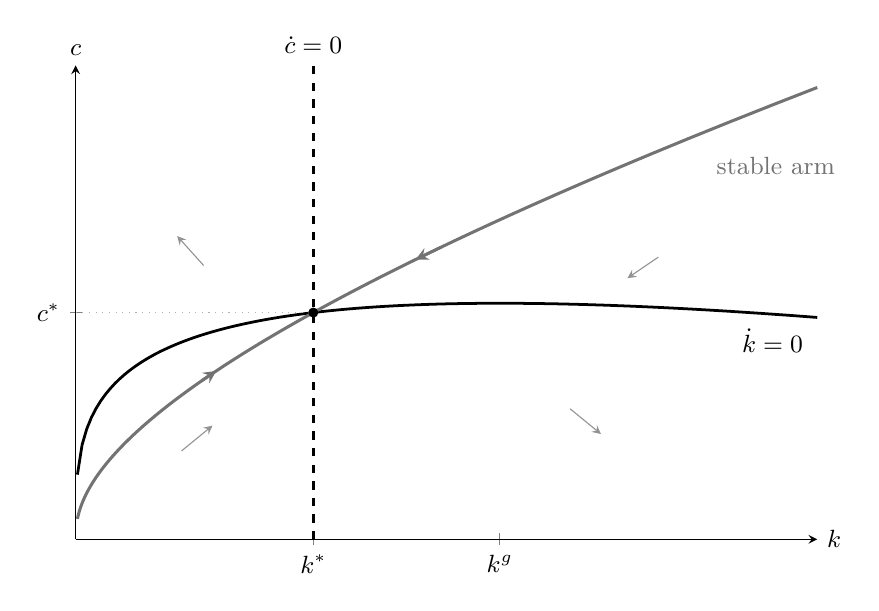
\begin{tikzpicture}
	\begin{axis}[
			width=11cm, height=7.6cm,
			axis lines=left,
			xlabel={$k$}, ylabel={$c$},
			every axis x label/.style={at={(current axis.right of origin)},anchor=west},
			every axis y label/.style={at={(current axis.above origin)},anchor=south},
			xmin=0, xmax=8.4, ymin=0, ymax=2.25,
			xtick={2.6918,4.8040}, xticklabels={$k^{\ast}$,$k^{g}$},
			ytick={1.0767}, yticklabels={$c^{\ast}$},
			tick label style={font=\small},
			label style={font=\small},
			clip=false,
		]

		% ---- the locus \dot k = 0, that is c = f(k) - \delta k ----
		\addplot[line width=1pt, domain=0.02:8.4, samples=160] {x^0.3 - 0.1*x};
		\node[anchor=north east, font=\small] at (axis cs:8.35,1.045) {$\dot k=0$};

		% ---- the locus \dot c = 0, that is f'(k) = \rho + \delta ----
		\addplot[line width=1pt, dashed] coordinates {(2.6918,0) (2.6918,2.25)};
		\node[anchor=south, font=\small] at (axis cs:2.6918,2.26) {$\dot c=0$};

		% ---- guide line to the steady state ----
		\addplot[gray!60, dotted] coordinates {(0,1.0767) (2.6918,1.0767)};

		% ---- the stable manifold, computed ----
		\addplot[line width=1.1pt, black!55] table {
				0.020000 0.096977
				0.022191 0.101387
				0.024900 0.106534
				0.027929 0.111952
				0.031460 0.117892
				0.035262 0.123913
				0.039508 0.130253
				0.044247 0.136930
				0.049536 0.143964
				0.055432 0.151372
				0.062002 0.159173
				0.069628 0.167727
				0.077805 0.176399
				0.086896 0.185529
				0.096997 0.195142
				0.108216 0.205266
				0.120660 0.215922
				0.134449 0.227135
				0.149681 0.238906
				0.167189 0.251762
				0.185750 0.264724
				0.206146 0.278297
				0.228535 0.292508
				0.253055 0.307365
				0.279859 0.322884
				0.309099 0.339077
				0.342279 0.356655
				0.376980 0.374259
				0.414574 0.392556
				0.455218 0.411555
				0.499012 0.431236
				0.546059 0.451585
				0.596432 0.472579
				0.652430 0.495074
				0.709714 0.517282
				0.770338 0.540008
				0.834243 0.563199
				0.901249 0.586768
				0.971145 0.610628
				1.043653 0.634680
				1.121499 0.659792
				1.198224 0.683895
				1.276326 0.707833
				1.355326 0.731489
				1.434651 0.754727
				1.513747 0.777425
				1.592066 0.799472
				1.672155 0.821608
				1.747312 0.842031
				1.820223 0.861541
				1.890527 0.880087
				1.957892 0.897627
				2.022073 0.914138
				2.082887 0.929611
				2.140222 0.944052
				2.196072 0.957989
				2.246122 0.970373
				2.292626 0.981793
				2.335634 0.992282
				2.375237 1.001881
				2.411548 1.010634
				2.444707 1.018586
				2.475999 1.026057
				2.503181 1.032520
				2.527686 1.038326
				2.549678 1.043520
				2.569328 1.048147
				2.586806 1.052253
				2.602282 1.055881
				2.616425 1.059189
				2.628311 1.061965
				2.638673 1.064381
				2.647653 1.066473
				2.655390 1.068273
				2.662012 1.069812
				2.667643 1.071120
				2.672568 1.072263
				2.676517 1.073179
				2.679793 1.073939
				2.682485 1.074563
				2.684673 1.075070
				2.686431 1.075477
				2.687825 1.075800
				2.688915 1.076052
				2.689782 1.076253
				2.690406 1.076397
				2.690866 1.076504
				2.691196 1.076580
				2.691426 1.076634
				2.691581 1.076669
				2.691680 1.076692
				2.691741 1.076706
				2.691774 1.076714
				2.691790 1.076718
				2.691797 1.076719
				2.691800 1.076720
				2.691800 1.076720
				2.691800 1.076720
				2.691801 1.076720
				2.691803 1.076721
				2.691808 1.076722
				2.691823 1.076725
				2.691851 1.076732
				2.691904 1.076744
				2.691992 1.076764
				2.692138 1.076798
				2.692351 1.076848
				2.692659 1.076919
				2.693091 1.077019
				2.693680 1.077155
				2.694466 1.077337
				2.695492 1.077574
				2.696812 1.077880
				2.698558 1.078284
				2.700664 1.078771
				2.703264 1.079372
				2.706441 1.080106
				2.710286 1.080994
				2.714898 1.082059
				2.720391 1.083326
				2.727170 1.084888
				2.734849 1.086657
				2.743818 1.088721
				2.754237 1.091115
				2.766284 1.093879
				2.780146 1.097056
				2.796037 1.100690
				2.814964 1.105009
				2.835723 1.109735
				2.859274 1.115083
				2.885916 1.121114
				2.915978 1.127897
				2.949813 1.135503
				2.987818 1.144012
				3.032234 1.153910
				3.080125 1.164527
				3.133631 1.176324
				3.193325 1.189406
				3.259837 1.203887
				3.333851 1.219886
				3.416136 1.237534
				3.511390 1.257790
				3.613229 1.279247
				3.726153 1.302810
				3.851284 1.328649
				3.989854 1.356947
				4.143206 1.387896
				4.312842 1.421706
				4.500403 1.458599
				4.716419 1.500491
				4.946328 1.544419
				5.200231 1.592197
				5.480543 1.644113
				5.789903 1.700472
				6.131251 1.761604
				6.507805 1.827863
				6.940567 1.902614
				7.400274 1.980527
				7.907069 2.064798
				8.400000 2.145277
			};
		\node[anchor=north west, font=\small, black!55] at (axis cs:7.15,1.86)
		{stable arm};

		% ---- steady state ----
		\filldraw (axis cs:2.6918,1.0767) circle (1.6pt);

		% ---- directional arrows in the four regions ----
		\draw[->,>=stealth,gray!85] (axis cs:1.45,1.30) -- (axis cs:1.15,1.44);
		\draw[->,>=stealth,gray!85] (axis cs:1.20,0.42) -- (axis cs:1.55,0.54);
		\draw[->,>=stealth,gray!85] (axis cs:6.60,1.34) -- (axis cs:6.25,1.24);
		\draw[->,>=stealth,gray!85] (axis cs:5.60,0.62) -- (axis cs:5.95,0.50);

		% ---- arrows along the stable arm, pointing towards the steady state ----
		\draw[->,>=stealth,black!55,line width=1pt]
		(axis cs:1.434651,0.754727) -- (axis cs:1.592066,0.799472);
		\draw[->,>=stealth,black!55,line width=1pt]
		(axis cs:4.143206,1.387896) -- (axis cs:3.851284,1.328649);
	\end{axis}
\end{tikzpicture}

	\caption[Phase diagram of the Ramsey problem]{The two loci of
		\autoref{thm:keynes-ramsey} and the stable manifold of
		\autoref{rem:ct-saddle-path}. Consumption rises to the left of $k^{\ast}$
		and falls to its right; capital rises below the hump and falls above it.
		The grey arrows give the direction of motion in each of the four regions.
		The modified golden rule places $k^{\ast}$ strictly below the golden-rule
		stock $k^{g}$ at which $f'(k)=\delta$, the wedge being the rate of time
		preference $\rho$.}
	\label{fig:ramsey-phase}
\end{figure}

\section{Chapter Summary}\label{sec:ct-summary}

Continuous-time optimisation replaces the choice of a sequence by the choice of a
path, and the first-order condition accordingly holds against every admissible
perturbation. The fundamental lemma converts such a family of integral conditions
into a pointwise differential equation, and it is the single analytic tool behind
all three methods presented.

The calculus of variations perturbs the path directly and yields the
Euler--Lagrange equation $f_x=\deriv{}{t}f_{\dot x}$, a second-order differential
equation matched to two endpoint conditions. It is necessary, not sufficient;
concavity of $f$ in $(x,\dot x)$ upgrades it to sufficient. Optimal control
separates the control from the state and perturbs the control, producing the
Hamiltonian $\mathcal{H}=f+\lambda g$ and three conditions --- optimality in the
control, a differential equation for the co-state, and the state equation ---
together with $\lambda(t_1)=0$ when the terminal state is free. The co-state is
the shadow price of the state, and the co-state equation is a no-arbitrage
condition on that price. The current-value Hamiltonian removes the discount factor
from the equations and leaves an autonomous system whose phase diagram carries
the dynamics. The calculus of variations is the case $g=u$. Dynamic programming
gives the Hamilton--Jacobi--Bellman equation
$\rho V(x)=\max_u\{r(x,u)+V'(x)g(x,u)\}$, in which the co-state is identified as
$V'(x)$; the heuristic passage from discrete time assumes differentiability of
the value function, and the rigorous route is verification against a candidate.

The continuous-time cake-eating problem yields $c=rk$, $k(t)=k_0e^{-rt}$ by all
three methods, and matches the discrete-time policy $c=(1-\beta)w$ in the limit
of short periods. In each derivation the first-order conditions leave one free
constant and only the transversality condition fixes it. The continuous-time
Ramsey model yields the Keynes--Ramsey rule
$\dot c/c=(f'(k)-\delta-\rho)/\gamma$ and the modified golden rule
$f'(k^{\ast})=\rho+\delta$, which places capital strictly below the golden-rule
level by the amount of impatience; the steady state is a saddle, and initial
consumption is the unique level placing the economy on the stable manifold.

\begin{exercise}\label{ex:ct-1}
	Prove \autoref{lem:fundamental-cov} under the weaker hypothesis that
	\eqref{eq:fundamental-cov} holds only for infinitely differentiable $h$
	supported in $(t_0,t_1)$, by replacing the quadratic bump with
	$h(t)=\exp\bigl(-1/((t-\alpha)(\beta-t))\bigr)$ on $[\alpha,\beta]$ and $0$
	elsewhere, and verifying that this $h$ is smooth. Explain why the strengthening
	matters for problems in which the admissible perturbations are constrained.
\end{exercise}

\begin{exercise}\label{ex:ct-2}
	Solve $\max\int_0^{T}e^{-\rho t}u(c)\,\diff t$ subject to $\dot a=ra-c$,
	$a(0)=a_0$ and $a(T)=0$, with $u(c)=c^{1-\gamma}/(1-\gamma)$. Show that
	$\dot c/c=(r-\rho)/\gamma$, solve for $c(0)$ from the terminal condition, and
	verify that the solution converges as $T\to\infty$ to the infinite-horizon
	solution under the transversality condition
	$\lim_{t\to\infty}e^{-\rho t}u'(c(t))a(t)=0$. Identify precisely where the
	terminal condition $a(T)=0$ replaces $\lambda(T)=0$ of
	\autoref{thm:maximum-principle} and why both cannot be imposed.
\end{exercise}

\begin{exercise}\label{ex:ct-3}
	Consider the Hotelling problem $\max\int_0^{\infty}e^{-\rho t}p(t)q(t)\,\diff t$
	subject to $\dot S=-q$, $S(0)=S_0$, where $p(t)$ is a given price path and
	$q\geq0$ is extraction. Show that the maximum principle gives
	$\dot\mu=\rho\mu$, so the shadow price of the resource grows at the rate of
	interest, and deduce Hotelling's rule that the price of the extracted resource
	net of extraction cost must grow at rate $\rho$ along any interior path. State
	what fails when extraction is constrained to a capacity $q\leq\bar q$, and
	relate the answer to \autoref{rem:which-bind}.
\end{exercise}
